% My first latex document.
% Author: Hilduara Abreu
%%%%%%%%%%%%%%%%%%%%%%%%%%%%%%%%%%%%%%%%%%%%%%%%%%%%%%%%%%%%%%%%%%%%%%%%%%%%%%%%%%%%%%%%%%%
\documentclass[11pt, letterpaper]{article}
\usepackage[margin=1in]{geometry}
\usepackage{fancyhdr}
\usepackage{fancyheadings}
\usepackage{titlepic}
\usepackage{pdfpages}
\usepackage[T1]{fontenc}
\usepackage{helvet}
\usepackage{fontawesome}
\usepackage[colorlinks=true, urlcolor=blue, linkcolor=blue]{hyperref}
\usepackage{graphicx}
\usepackage[mmddyyyy]{datetime}
\usepackage{fancyhdr}
\setlength{\parskip}{2mm}
\setlength{\parindent}{0mm}
\setcounter{secnumdepth}{3}
\setcounter{tocdepth}{3}
\usepackage{setspace}
\usepackage{wrapfig}
\hypersetup{breaklinks=true}
\usepackage{verbatim}
\usepackage{fvextra}
\usepackage{float}
\usepackage{lipsum}
\usepackage{xurl}


% Cover Page
%%%%%%%%%%%%%%%%%%%%%%%%%%%%%%%%%%%%%%%%%%%%%%%%%%%%%%%%%%%%%%%%%%%%%%%%%%%%%%%%%%%%%%%%%%%%%%%%%%

\begin{document}
\sloppy
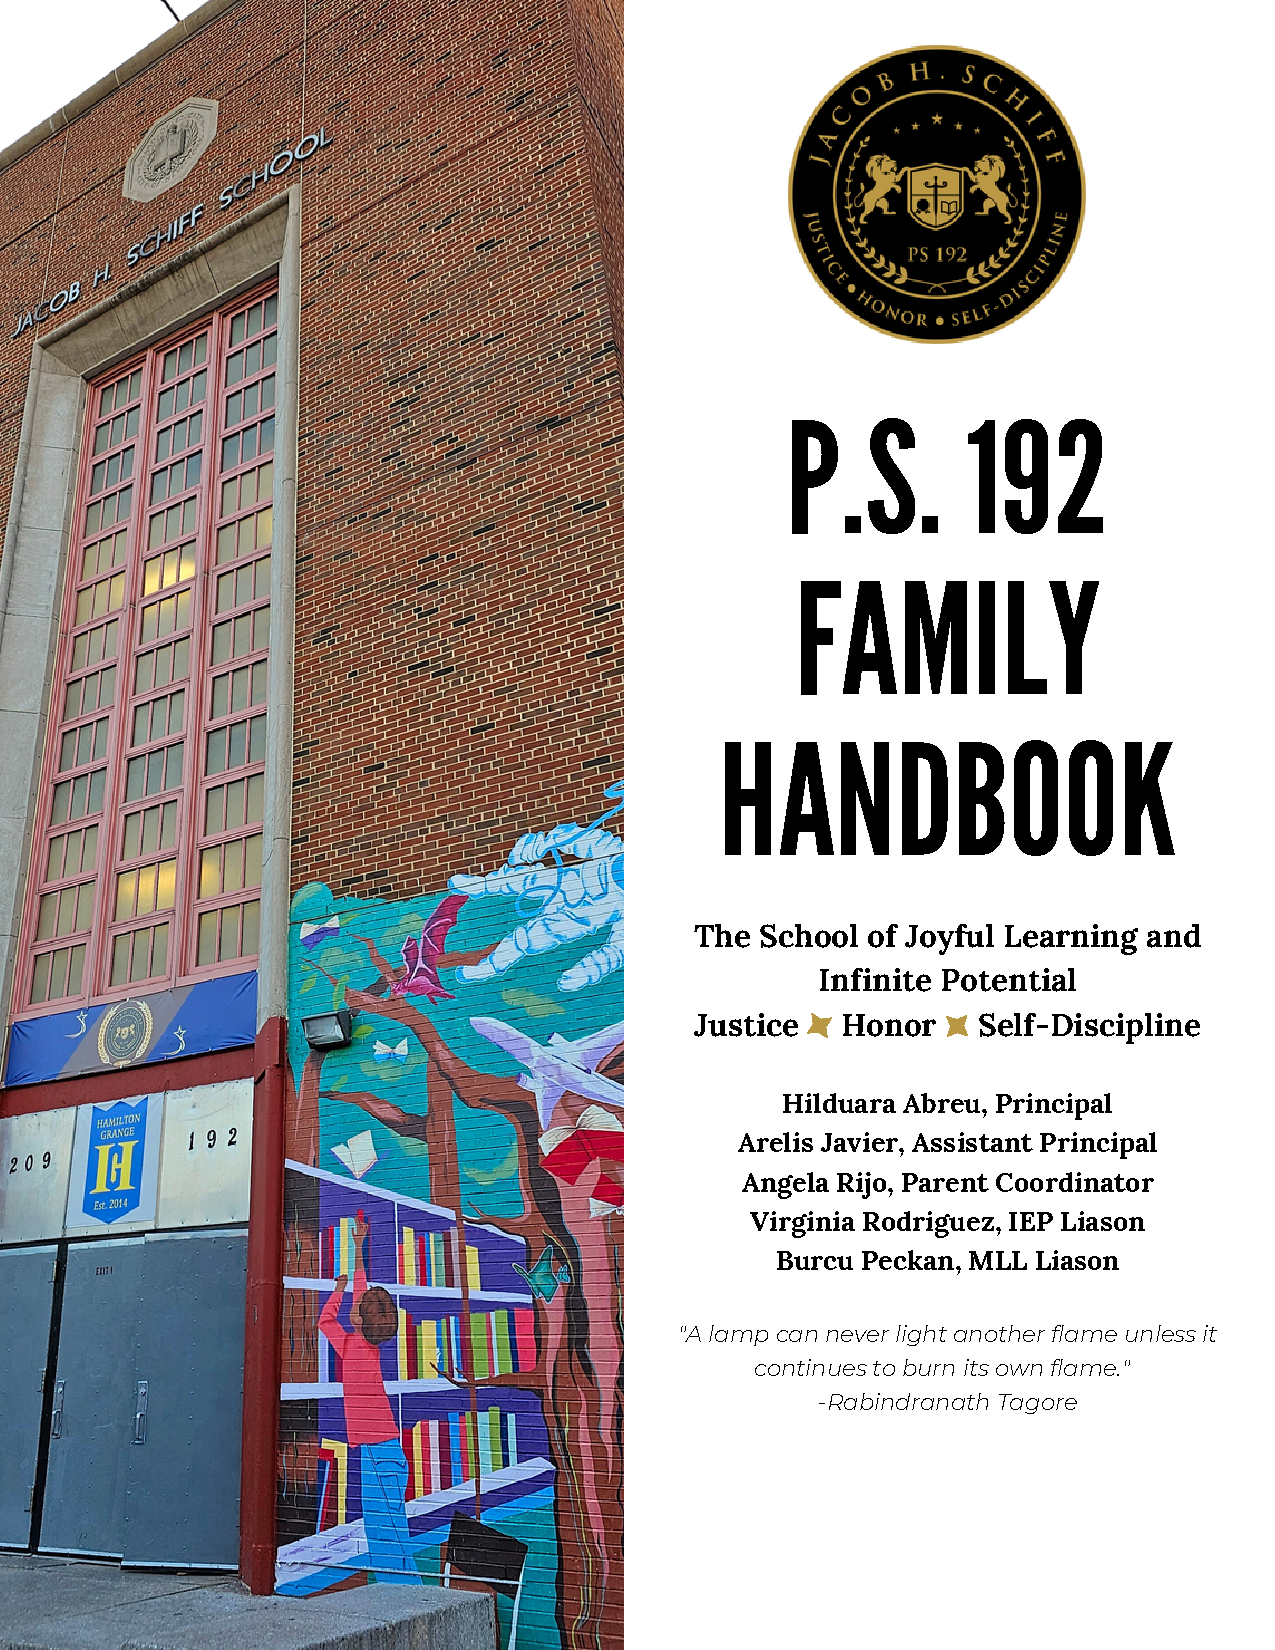
\includepdf[pages=1,fitpaper]{handbook_front.pdf}

%%%%%%%%%%%%%%%%%%%%%%%%%%%%%%%%%%%%%%%%%%%%%%%%%%%%%%%%%%%%%%%%%%%%%%%%%%%%%%%%%%%%%%%%%%%%%%%%%%

% Header & Footer
\pagenumbering{\fancyhf{}}
\pagestyle{headings}
\pagenumbering{arabic}
\fancyhead[L]{\textit{Staff Handbook 2023-2024}}
\fancyhead[R]{\thepage}
\fancyfoot[C]{The School of Joyful Learning!}
\pagestyle{fancy}
\renewcommand{\footrulewidth}{1 px}

% TOC
%%%%%%%%%%%%%%%%%%%%%%%%%%%%%%%%%%%%%%%%%%%%%%%%%%%%%%%%%%%%%%%%%%%%%%%%%%%%%%%%%%%%%%%%%%%%%%%%%%

\newpage
\tableofcontents
% \thispagestyle{empty}
\newpage

% Begin Documents
%%%%%%%%%%%%%%%%%%%%%%%%%%%%%%%%%%%%%%%%%%%%%%%%%%%%%%%%%%%%%%%%%%%%%%%%%%%%%%%%%%%%%%%%%%%%%%%%%%
\section{Message from The Principal}
Welcome to \href{https://www.ps192.org}{P.S. 192}, where excellence in education is not just a goal, but a way of life. It is with immense pleasure and pride that I extend my warmest greetings to you all as we embark on yet another exciting academic year.

At \href{https://www.ps192.org}{P.S. 192}, we are more than just an educational institution; we are a community united by a shared vision of nurturing young minds and shaping future leaders. Our school's emblem, proudly displaying the noble lion and lioness, symbolizes the strength, courage, and unwavering determination that define our journey together.

As we journey forward, we remain steadfast in our commitment to instill three core values into the hearts of our students: Justice, Honor, and Self-Discipline. These values are the guiding principles that underpin everything we do. They form the bedrock upon which we build character, foster empathy, and cultivate the leaders of tomorrow.

In the pages of this Family Handbook, you will find a wealth of information about our school's policies, programs, and opportunities. It is designed to be your compass, helping you navigate the rich and rewarding educational experience we offer.

Together, as a united educational family, we will empower your child to explore their potential, embrace challenges, and emerge as confident, compassionate, and responsible individuals ready to make a positive impact on the world.

Thank you for entrusting us with the privilege of shaping your child's future. Together, we will roar with pride as our students become the lions and lionesses of tomorrow, embodying the values of justice, honor, and self-discipline.

Respectfully yours,


\includegraphics[width=0.2\textwidth]{hil_signature}

Hilduara Abreu

Principal

\textbf{The School of Joyful Learning!}
\pagebreak
\begin{wrapfigure}{L}{0.5\textwidth}
\centering

\includegraphics[width=.45\textwidth]{positivity.pdf}
\end{wrapfigure}
\section{About P.S. 192 | Jacob H. Schiff School}
Welcome to P.S. 192 | Jacob H. Schiff School, where we believe in nurturing "Infinite Potential" in every child. Our school is more than just a place of learning; it's a community dedicated to unlocking the limitless abilities and intelligence within each of our students through dedication, learning, and resilience. We are committed to instilling core values of justice, honor, and self-discipline in every aspect of our educational journey.

\subsection{History}
Our school was established in 1952, was once home to the Hebrew Orphan Asylum of New York (HOA). It began as a modest educational institution serving the local community.

Jacob H. Schiff's contributions extended beyond our school, as he actively supported various initiatives that aimed to uplift marginalized communities, promote civil rights, and advance educational opportunities. His commitment to justice and social equity has left an enduring impact on our institution and our community.

\subsection{Our Commitment}
At P.S. 192, we foster a dynamic and engaging learning environment. Our experienced educators are dedicated to providing personalized support to each student, recognizing that every child has unique strengths and areas for growth. We encourage curiosity, creativity, and critical thinking, empowering our students to tackle challenges as opportunities for growth and discovery.

\subsection{Core Values}
\begin{itemize}
\item Justice: At P.S. 192, we teach our students the importance of fairness and equity. We instill a sense of social responsibility, encouraging them to be advocates for justice in their school, community, and the world.
\item Honor: We emphasize the value of integrity and respect. Our students learn the importance of honesty, trustworthiness, and treating others with dignity, ensuring they carry these principles throughout their lives.
\item Self-Discipline: Self-discipline is a cornerstone of personal growth. We guide our students in developing strong work ethics and the ability to set and achieve goals. We believe that self-discipline is the key to unlocking their infinite potential.
\end{itemize}

\subsection{Infinite Potential}
"Infinite Potential" is not just a slogan; it's a guiding philosophy at P.S. 192 | Jacob H. Schiff School. We believe that every child possesses boundless possibilities waiting to be unlocked. By nurturing their potential and instilling the values of justice, honor, and self-discipline, we prepare them to succeed academically, socially, and morally.

\subsection{Mission}
To provide a welcoming, safe, resourceful, and nurturing environment that supports our school community's academic and social-emotional development where children are respected and engaged in challenging curricula that motivate them to realize their potential as active, lifelong learners. Through our guiding core values of Justice, Honor, and Self-discipline, we aspire to promote perseverance, love, empathy, and respect for oneself and others.

\subsection{Vision}
To ensure all students acquire the essential knowledge and skills they need to become independent thinkers and become active participants and contributors in their roles as students and as members of society.

\begin{wrapfigure}{L}{.5\textwidth}
\centering

\includegraphics[width=.4\textwidth]{himher7.png}
\end{wrapfigure}

\subsection{School Motto}
"Good, better, best. Never let it rest until your good is better, and your better is best." | St. Jerome

\subsection{School-Wide Norms of Conduct}
P.S. 192 follows school-wide norms which is the daily recitation of the Positivity Pledge every morning.

\subsection{Our Teaching Staff}
P.S. 192 prides itself on the quality of our teachers. Our teaching staff is diverse with a variety of skills and expertise. Teachers work together sharing talents and strengths to maximize learning and opportunities for students.

Our faculty includes 12 classroom teachers, a physical education teacher, two ENL teachers, a Science teacher, an IEP Liason. We have two arts teachers on faculty specializing in Visual Arts and Music and bring in consultants to teach Dance and Drama. Our Social Workers  and school psychologist help students with social and emotional development. We often host student teachers from City College and Columbia University’s Teachers College. Lastly we have a robust staff of paraprofessionals speech pathologists, an occupational therapist, and a physical therapist who work with our teachers to provide individualized support.
\begin{wrapfigure}{R}{.7\linewidth}

\includegraphics[width=.85\linewidth]{logohim.png}
\end{wrapfigure}
\section{Looping Model \& Curricula}
\subsection{Looping Model}
Looping is a practice where a teacher stays with the same group of students for more than one school year, fostering a continuous and supportive learning environment. Here's why it's crucial for your child's education:
\begin{itemize}
\item \textbf{Strong Teacher-Student Relationships:} Looping allows teachers to develop deeper bonds with students. They understand each child's unique learning style, strengths, and areas of improvement, resulting in a more tailored educational experience.
Consistency and Stability: By staying together, students and teachers create a stable and familiar classroom environment. This reduces anxiety, encourages active participation, and enhances the overall learning experience.
\item \textbf{Seamless Transition:} Moving from one grade to another can be challenging for children. Looping eases this transition as students remain with a familiar teacher, minimizing disruptions and ensuring a smoother academic journey.
\item \textbf{Academic Growth:} Teachers can build on the knowledge gained in the previous year, enabling a more fluid progression of skills and concepts. This often leads to improved academic outcomes.
\item \textbf{Personalized Support:} With a deeper understanding of each student's needs, looping teachers can provide targeted interventions and support, ensuring that every child reaches their full potential.
\end{itemize}
As parents, your involvement and support are vital to the success of the looping process. We encourage you to communicate regularly with your child's teacher and stay engaged in their educational journey.

\subsection{Curricula}
\textbf{Exploring the World Through Expeditionary Learning, enVision, Passport-to-Social-Studies, Amplify Science \& Sanford Harmony}

At \href{https://www.ps192.org}{P.S. 192} | Jacob H. Schiff, we are committed to providing your child with an enriching and dynamic educational experience. One of the exciting approaches we use to ignite their curiosity and love for learning is Expeditionary Learning!
\begin{itemize}
 \item \textbf{Expeditionary Learning}
\begin{itemize}
\item The EL Education curriculum is founded on the principles of the Science of Reading, incorporating systematic phonics instruction to enable every student to proficiently read challenging grade-level materials and attain mastery of literacy standards, thereby ensuring equitable educational outcomes for all students.
\item Our educational program fosters profound understanding through the incorporation of content-rich, genuine texts related to real-world subjects encompassing social studies, STEM, and literature. Students utilize their acquired knowledge to advocate for social justice and environmental responsibility, concurrently cultivating virtuous attributes that empower them to make meaningful contributions to the improvement of society.
\end{itemize}
\item \textbf{Envision}
\begin{itemize}
\item This instructional tool finds application in classrooms worldwide. enVision Mathematics places its emphasis on fostering a profound conceptual grasp of mathematics through the utilization of visual models, personalized instruction, and the implementation of 3-act tasks. Additionally, Family Engagement resources are made available to offer indispensable information to families, enabling them to support their students in their home learning endeavors. Furthermore, the program offers a comprehensive vertical alignment spanning from Kindergarten through Algebra 2, enabling schools to effectively address and meet mathematical standards.
\end{itemize}
\item \textbf{Passport-to-Social-Studies}
\begin{itemize}
\item This program prompts students to adopt a historical mindset, urging them to pose inquiries, engage in critical thinking, explore various viewpoints, and amass substantiating evidence to underpin their analyses. This is achieved through the cultivation of skills in chronological analysis, decision-making, and the rigorous pursuit of historical research and examination.
\end{itemize}
\item \textbf{Amplify Science}
	\begin{itemize}
	\item Students assume the role of scientists or engineers as they actively explore captivating phenomena through interactive hands-on exercises, immersive digital simulations, extensive reading and writing tasks, and dynamic classroom discussions.
	\end{itemize}
\item \textbf{Sanford Harmony}
	\begin{itemize}
	\item The socio-emotional program fosters enhanced classroom relationships, allowing educators to allocate less effort to the management of disruptive classroom conduct and dedicate more time to instruction.
	\end{itemize}
\end{itemize}

\begin{figure}[H]
  \centering

\includegraphics[width=1\linewidth]{1.png}
\caption{\textbf{The School of Joyful Learning!}}
  \label{fig:PS192}
\end{figure}

It's a journey of discovery that allows your child to explore the world, develop critical skills, and grow as a well-rounded individual. Here's why we believe the aforementioned curricula provide remarkable opportunities for our students: 
\begin{itemize}
\item \textbf{Real-World Learning:} Expeditionary Learning exposes students to real-life experiences and challenges. Instead of just reading about science, history, or nature, your child will get the chance to see, touch, and experience it firsthand. Whether it's a field trip to a science museum, a historical reenactment, or exploring the local environment, they will connect classroom knowledge to the world around them.
\item \textbf{Critical Thinking and Problem-Solving:} Our expeditions encourage students to think critically, ask questions, and solve problems independently. They'll learn to work as a team, make decisions, and adapt to different situations. These skills are not only essential for academic success but also for lifelong learning.
\item \textbf{Empathy and Social Awareness:} Expeditionary Learning promotes social and emotional growth. By interacting with diverse groups of people and communities, your child will develop empathy and a deeper understanding of the world's complexities. This fosters a sense of responsibility and global citizenship.
\item \textbf{Passion and Engagement:} When students are actively involved in their learning, they become more passionate about it. Expeditionary Learning taps into your child's natural curiosity, making education exciting and enjoyable.
\item \textbf{Stronger Community Bonds:} Through expeditions, your child will build strong bonds with classmates, teachers, and the community. These connections provide a support system that enhances their overall educational experience.
\item \textbf{Personal Growth:} As your child faces challenges and overcomes obstacles during their expeditions, they'll develop confidence and resilience. These personal growth experiences are invaluable for their future success.
\item \textbf{Lifelong Love for Learning:} Ultimately, Expeditionary Learning helps foster a lifelong love for learning. By making education an adventure, we inspire our students to continue exploring and discovering throughout their lives.
\end{itemize}
We are excited to embark on this learning journey with your child and hope you'll join us in supporting their explorations. Keep an eye out for information about upcoming expeditions and ways you can get involved.

If you have any questions or would like to learn more about Expeditionary Learning at \href{https://www.ps192.org}{P.S. 192}, please don't hesitate to reach out to our dedicated staff.

Together, we'll empower your child to explore, learn, and grow as they discover the world around them!

In addition, we partner with numerous organizations each year to bring in skills and expertise from a variety of fields. Partnerships often help shape our curriculum. Some of our partnerships have included Mission Society	, Project Tomorrow, Creative Art Works, Matheka and the ETM - Education through Music. 

\begin{figure}[H]
  \centering

\includegraphics[width=1\linewidth]{2.png}
\caption{\textbf{The Lion's Den}}
  \label{fig:school mascots}
\end{figure}

\subsection{Response to Intervention (RTI)}
At \href{https://www.ps192.org}{P.S. 192}, we are committed to instructing all our students in accordance with their optimal learning methods. Occasionally, students may require supplementary or diversified academic assistance to realize their full academic capabilities. Consequently, our academic intervention strategies at \href{https://www.ps192.org}{P.S. 192} are aligned with the principles of Response to Intervention (RtI), a structured framework designed to optimize student growth throughout all grade levels. For further information regarding RtI and the educational policies of New York City and State, we invite you to explore nysrti.org.

\section{Assessment of Student Work}

\subsection{Reporting Student Progress}

Our grading policy is below as Appendix 3.

\subsubsection{Homework Policy}
We aspire for our students to cultivate their cognitive abilities, evolve into independent scholars, and identify themselves as accomplished learners. We firmly endorse the idea that homework serves as a catalyst for developing commendable habits such as effective time management, self-reliance, and organizational skills. Homework serves as a medium to convey the fundamental notion that the pursuit of knowledge, exploration, and introspection extends beyond the confines of the school environment. Furthermore, it accentuates the significance of familial involvement by fostering dialogues between parents and children regarding information, thoughts, and diverse perspectives. In pursuit of these objectives, we meticulously design meaningful assignments, tailor tasks to individual needs, prioritize feedback, and implement strategies to enhance homework completion.

The purpose of homework in the P.S. 192 learning process is:
\begin{itemize}
\item Checking for understanding
\item Practicing
\item Processing
\item Pre-learning
\end{itemize}

All homework:
\begin{itemize}
\item Have a clear academic purpose,
\item Be customized for individual students,
\item Instill a sense of competence,
\item Be well-organized, easy to understand and visually pleasing.
\end{itemize}

To adhere to the recommended guidelines, we adhere to the "10-minute rule," signifying that the maximum daily homework duration corresponds to ten minutes per grade level. For instance, fifth-grade students should expect a maximum of 50 minutes of homework nightly. This practice aligns with the recommendations set forth by esteemed educational organizations, such as the National Education Association (NEA) and the National Parent Teacher Association (PTA). In addition to assigned tasks, we strongly encourage all students to engage in daily reading or listening to reading.

Should your child encounter instances of incomplete or delayed assignments, our educators will collaborate with you and your child to devise a remedial plan. Moreover, in cases where consistent challenges with homework completion arise, we will engage in a collaborative effort to explore effective strategies with both the student and parents. Our foremost objective is to diagnose and address any underlying issues that may hinder the timely completion of homework.

Your partnership in nurturing our students' commitment to learning is greatly valued, and we look forward to a successful academic journey ahead.

\subsubsection{Parental Involvement in Homework}
We encourage parental engagement in assisting their child with homework, with a primary emphasis on the child taking ownership of the work. Should you seek recommendations on how to best facilitate your child's progress, we kindly request that you reach out to their respective teacher for guidance and advice.

Kindly ensure to reach out to your child's teacher in the following circumstances:
\begin{itemize}
\item If your child encounters difficulties in completing their homework independently.
\item When homework becomes a source of distress for your child.
\item If the volume of homework is encroaching upon valuable sleep, recreational, or family time.
\item When homework begins to cultivate a negative sentiment towards school in your child.  
\end{itemize}

\begin{figure}[H]
  \centering

\includegraphics[width=1\linewidth]{4.png}
\caption{\textbf{"Today and every day, let justice guide your actions, honor inspire your choices, and self-discipline be the key to unlocking your potential. You are the future of a brighter, fairer world."}}
  \label{fig:school symbol}
\end{figure}

\subsection{Standardized Testing}
The No Child Left Behind Act necessitates that educational institutions annually conduct State assessments in English Language Arts and Mathematics for students in grades 3–8, as well as in Science at least once during grades 3–5 and 6–9.

In adherence to these statutory obligations, \href{https://www.ps192.org}{P.S. 192} School conducts the New York State English Language Arts (ELA) and Mathematics examinations for students in grades 3, 4, and 5, as well as the Science examination for grade 5 students on an annual basis. \href{https://www.ps192.org}{P.S. 192} administers these assessments in compliance with federal and state directives. It is important to note that these examinations are not utilized for the purpose of tracking individual students' year-to-year progress, determining class placement, or influencing promotion decisions.

While the majority of our school community participates in these assessments, we wish to emphasize that families retain the right to opt out of testing, and \href{https://www.ps192.org}{P.S. 192} fully supports their decision in this matter. Should a family opt for this choice, they are kindly requested to formally submit their request in writing to the principal at least one week prior to the scheduled testing date. In such cases, students who do not partake in the examinations will engage in meaningful educational activities related to the subject area being assessed.

We value the partnership between our school and our students' families, and we are committed to ensuring that all students have a conducive and enriching learning environment.

\section{Key Details for Families}
Your child's classroom teacher will serve as your main point of contact at the school. Below is a list of other individuals you may need to reach out to and the reasons for contacting them. You can contact any of them through the main school phone number during school hours

Main Office, \href{tel:2127759560}{(212) 775-9560}

\begin{table}[h]
\Large
\centering
\begin{tabular}{|l|l|l|}
\hline
\multicolumn{3}{|c|}{\textbf{P.S. 192- Jacob H. Schiff}}                                                                                                                                                      \\ \hline
\multicolumn{1}{|c|}{\textbf{Staff}} & \multicolumn{1}{c|}{\textbf{Position}} & \multicolumn{1}{c|}{\textbf{Contact}}                                                                                         \\ \hline
Hildura Abreu                        & Principal                              & \href{https://www.ps192.org/apps/pages/index.jsp?uREC_ID=1129573&type=u&pREC_ID=2364229}{contact page} \\ \hline
Arelis Javier                        & Assistant Principal                    & \href{https://www.ps192.org/apps/pages/index.jsp?uREC_ID=1199574&type=u&pREC_ID=2401120}{contact page} \\ \hline
Angela Rijo                          & Parent Coordinator                     & \href{https://www.ps192.org/apps/pages/index.jsp?uREC_ID=1199597&type=u&pREC_ID=2373071}{contact page} \\ \hline
Dulce Infante                        & Secretary                              & \href{https://www.ps192.org/apps/pages/index.jsp?uREC_ID=1974810&type=u}{contact page}                   \\ \hline
Luisa Estrella                       & Social Worker                          & \href{https://www.ps192.org/apps/pages/index.jsp?uREC_ID=1199562&type=u&pREC_ID=2397226}{contact page} \\ \hline
Virginia Rodriguez                   & IEP Liason (Special Education)         & \href{https://www.ps192.org/apps/pages/index.jsp?uREC_ID=2063032&type=u&pREC_ID=2365819}{contact page} \\ \hline
Burcu Peckan                         & ESL Liason                             & \href{https://www.ps192.org/apps/pages/index.jsp?uREC_ID=1199550&type=u}{contact page}                   \\ \hline
Sharlymet Cuesta                     & Family Worker                          & \href{https://www.ps192.org/apps/pages/index.jsp?uREC_ID=1199556&type=u}{contact page}                   \\ \hline
\end{tabular}
\caption{\textbf{P.S. 192 First Response Team}}
\label{tab:my-table}
\end{table}

\subsection{Meal Application Form}
All students within the jurisdiction of New York City are entitled to receive complimentary lunch services. Nevertheless, it is imperative that parents undertake the completion of the meal application form accessible at \href{https://www.myschoolapps.com/}{MySchoolApps}. The significance of this form lies in its role as a vital instrument through which the Department of Education (DOE) calculates a portion of the funding allocated to \href{https://www.ps192.org}{P.S. 192}.

To successfully fulfill this application, it is necessary to provide the following information:
\begin{itemize}
\item The names and income details of each member constituting your household.
\item Pertinent details regarding the school, grade, and birth-date of every student within your household.
\item The last four digits of your social security number along with an electronic signature.
\item A valid email address or phone number for communication with the Office of School Food concerning the status of your application.
\end{itemize}
Your prompt attention to and completion of this application is greatly appreciated and ensures the continued support of essential resources for \href{https://www.ps192.org}{P.S. 192}. For assistance, please reach-out our parent coordinator, \href{arijo@schools.nyc.gov}{Ms. Rijo}.

\subsection{Attendance and Lateness}
Consistent attendance plays a pivotal role in achieving success within our educational institution. Each instance of absence equates to a forfeiture of valuable instructional time and poses a potential risk to your child's academic progress, potentially causing them to lag behind in the acquisition of fundamental skills.

It is imperative to acknowledge that your child's attendance, encompassing punctuality as well, is meticulously documented as part of their permanent educational dossier. This attendance record is meticulously maintained within the Automated Schools (ATS), a real-time student data tracking system sanctioned by the New York City Department of Education (NYC DOE). The vigilance with which we monitor attendance underscores its significance, not only as an individual indicator but also as a substantial component contributing to the evaluation of our school's overall performance by the NYC DOE, which, in turn, holds us accountable to the highest educational standards.

Please be aware that in the event of excessive absences, the ATS system will automatically trigger the generation of a Form 407 Attendance Follow-up and Outreach Referral, followed by a scheduled home visit as a proactive measure.

For a more comprehensive understanding of our school's attendance policies and procedures, we invite you to consult the attached \hyperref[firstappendix]{P.S. 192 Attendance Policy}, which provides detailed information on this crucial aspect of your child's education. Your partnership in ensuring regular attendance is greatly appreciated, as it significantly contributes to your child's educational journey.

Should you have any inquiries or require further clarification, please do not hesitate to reach out to Principal Abreu. Together, we can provide the best educational experience for your child. 

\subsection{Arrival and Dismissal}
Our school commences its instructional day promptly at 8:00 AM, concluding at 2:20 PM. We kindly request your cooperation in ensuring your child's timely arrival at the beginning and prompt pickup at the end of the school day. Our dedicated school staff diligently uphold the safety and accountability of all children under their care at all times. It is of utmost importance that every family adheres to our established protocols for both drop-off and dismissal, as this is essential for us to maintain this high standard of safety. For further guidance on attendance and punctuality, please refer to the section below outlining the Department of Education's policies. Additionally, we have included an attached appendix on Attendance that provides comprehensive information regarding arrival, dismissal, and overall attendance procedures.

\subsection{Arrival}
Students can be dropped off at 8:00 AM for regular arrival or at 7:40 AM if they are having school breakfast. Students are dropped off either the cafeteria entrance or at the main entrance depending upon their grade and arrival time. Students arriving by bus are greeted by our Parent Coordinator, Ms. Rijo in front of the school as they disembark from the bus.

\subsection{Late Arrivals}
We kindly request your punctuality, as tardiness can disrupt the day to day operation of the school and potentially impact a child's educational progress. Each morning, our classes commence with a brief morning meeting followed by instructional activities. In the event that your child arrives late, the teacher will promptly inform the main office, where the tardiness is recorded in the ATS system.

Should your child arrive after the designated attendance submission time, typically around 8:30 am, you may receive an email notification from the Department of Education (DOE) indicating their absence. This occurs because all attendance records must be finalized by a specific time, and any changes made after this deadline will not be reflected in the system until the following morning. Your cooperation in ensuring timely arrivals is greatly appreciated.

Students should not miss school except in the case of illness. Please send a note to \href{mailto:scuesta@schools.nyc.gov}{scuesta@schools.nyc.gov} EACH time your child is absent. A doctor’s note is required after two (2) days.
  
\textbf{We strongly advise families to not schedule vacations when school is in session.}

We also request that every effort be made to schedule a doctor’s appointments \textbf{after school hours}. If this is not possible, please have your child attend for part of the day.  

\subsection{Dismissal}
Dismissal is at 2:20 PM Students are picked up outside inside the school yard. Please be prompt to pick up your child. Late pickups cause your child unnecessary anxiety, inconvenience teachers and jeopardize our ability to keep a safe school environment.

We can only release your child to adults designated on the emergency contact card or on the \href{https://www.schoolsaccount.nyc/ny}{NYCSA}  Parent Account. This applies even if it is another P.S. 192 family you are asking to pick up your child. If a teacher is not familiar with the person picking up, they may ask for ID to ensure that the person is on the list. 

Dismissal is not a time for a long conversation with staff. Staff must remain focused on the \textbf{safety of all their students}. If you need to speak with a staff member, please schedule a time to do so. You may send an email or a ClassDojo text to the child's teacher.

Please make every effort to be on time for pick up - staff have families to go home to or other work assignments. If you think you will be late for dismissal please call the main office to notify us as soon as possible so we can inform your child and relevant staff and so that we can plan for staff to stay with students if needed. Students who are still in their classroom or the yard 10 minutes after dismissal are taken to the main office and parents/guardians are called.

At the beginning of the year, you must fill out a dismissal form listing who will pick up your child each day. We also ask for their contact information in case they are late. Please make sure to update this form with the office if there are long term changes like new babysitters, after school programs, classes or clubs.

If there is a change to this dismissal information for the day, you must email \href{mailto:arijo@schools.nyc.gov}{arijo@schools.nyc.gov} before 11 AM the day of the change. (8 AM for half days.) This allows us enough time to make everyone involved in dismissal knows. Please do NOT communicate dismissal changes to teachers as they are not able to view their email during the school day.

Please plan ahead regarding changes in your pick up procedure. Frequent changes to dismissal plans can be unsettling to your child and disruptive to the class and school. 

\subsection{Early Dismissal}
If you are picking up your child please email us ahead of time at
\href{mailto:arijo@schools.nyc.gov}{arijo@schools.nyc.gov}. When you arrive, a staff member will bring your child to you and have you sign the early pick up book. Only authorized adults may sign out a student. Even if your student is an independent walker, they must be picked up by an adult if they are leaving before the end of the school day. Early dismissal MUST be before 1:30 PM. If you are not here before 2:00 PM you must wait until regular dismissal at 2:20 PM.

\subsection{Transportation}
If you want to know if your child is eligible for the school bus or a metro card please contact our Parent Coordinator, Ms. Rijo. The FAQ: \hyperref[secondappendix]{Bus and Metro Card}

\subsection{Wellness and Healthy Eating}
P.S. 192 is committed to promoting healthy lifestyles and providing educational opportunities to learn about nutrition, physical fitness and taking care of ourselves.

\subsection{Breakfast/Lunch/Snack} 
Eating a good breakfast is essential to have a great day in school. Breakfast is free to all students and is available starting at 7:40 AM. 

P.S.192's lunch and recess period begins at 10:30 AM. School lunch is free for all students. Students may choose to bring lunch from home. No refrigeration is available for lunches brought from home. 
\begin{itemize}
\item \textbf{NUTS:} There are some children in our building who are severely allergic to nuts. To ensure all of our student's health and safety, P.S. 192's have a policy of no nuts in lunches or snacks. 
\item \textbf{NO JUNK FOOD:} Do not send any type of candy, chips, cookies or sugary drinks for your child’s lunch or snack. Gum chewing is not allowed unless arranged with a classroom teacher as part of a sensory need.
\end{itemize}

The menus for school breakfast and lunch are available on the DOE website at: \href{https://www.schools.nyc.gov/school-life/food/menus}{NYC School Food Menu}.  

\subsection{Recess}
All children have a supervised recess either before or after lunch. Kindergarten through 2nd grade students play first then eat. 3rd-5th graders eat first and then play. We take the children outside for recess, even in the winter, unless it is raining or the temperature or wind chill is particularly cold (below 32 degrees F). Children must have appropriate outerwear. This includes hats, scarves, gloves and boots if necessary. \textbf{All items must be labeled with your child’s name}.

\subsection{Dressing for Success}
Students should wear comfortable clothing and shoes that they can be active in. Students are likely to use paint, markers and glue several times a week. School activities often require sitting on the rug or floor. Please avoid fancy clothing that "cannot get dirty.” Please send your child in sneakers or other sturdy shoes. Platform shoes, shoes with a heel, flip flops, loose sandals, and tight clothing can all limit a child’s ability to run as well as their safety on the climbing equipment.

Our building has central air conditioning which makes it difficult to regulate the temperature in individual classrooms. Even when it is very hot outside, make sure your child has a sweater or sweatshirt to ensure they are comfortable in the classroom.  

Kindergarten and 1st grade - In the first week of school, please bring an extra set of clothing for your child, labeled and in a ziploc bag.

\subsection{Remote and Online Learning}
\href{https://www.ps192.org}{P.S. 192} employs Google Classroom for the facilitation of homework assignments and remote learning. It is important to note that remote learning will be implemented in the event of inclement weather, such as snow days. Specifically, within the upper-grade levels, notably the 5th grade, students utilize Google Docs and slides as tools to accomplish assignments both within the school premises and in the comfort of their homes.

\subsection{Remote and Online Learning}
The primary login portal for all Department of Education (DOE) programs is located at \href{https://www.ps192.org}{TeachHub}. Your student will complete the sign-in process, after which the homepage can be tailored to incorporate the most frequently utilized applications. It is important to note that upon enrollment in the DOE, all students are provided with a DOE email address and corresponding login credentials.

By means of the \href{https://www.ps192.org}{TeachHub} platform, your child is granted access to Google Classroom, along with the suite of Google applications such as Docs. Additionally, students have the opportunity to utilize Sora for reading, provided through the New York Public Library, as well as Zoom for participating in online classes during remote learning sessions.

\subsection{Technology}
Given the shift towards remote learning, it is imperative that every student possesses either an iPad or a laptop to facilitate their engagement in at-home remote learning. Should your child lack access to such a device, please be advised that \href{https://www.ps192.org}{P.S. 192} will extend the provision of one device per student on an annual basis. Additionally, in cases where an internet connection is unavailable within your home, we shall furnish a device equipped with built-in internet connectivity.

For any inquiries or concerns pertaining to devices or technological matters, we kindly request you to reach out to \href{mailto:ajavier@schools.nyc.gov}{Ms. Javier}. Your questions and requirements will be addressed with utmost care and attention.

\subsection{Birthdays}
Monthly, we come together during our Town Meeting to commemorate birthdays, fostering a sense of community and inclusivity within our school. Individual classroom birthday celebrations are not conducted. Instead, our dedicated teachers employ special methods to recognize and honor each child on their special day. This may include mentioning the student's name during the morning greeting or reading their favorite book.

In addition to these personalized acknowledgments, as a united class community, we gather for a collective monthly celebration at the conclusion of each month. During this gathering, families of birthday celebrants are welcome to provide a special snack.

For those with summer birthdays, we come together to celebrate in the month of June. In line with our commitment to promoting healthy habits, we kindly request that families adhere to our healthy eating guidelines, refraining from including goody bags or candy as part of the celebration. Furthermore, teachers have the flexibility to choose between utilizing the outdoor yard or their classroom space for these gatherings, ensuring a memorable and enjoyable experience for all.

Our approach to birthdays reflects our dedication to fostering a supportive and health-conscious learning environment while creating lasting memories for our students.

\subsection{Lost and Found}
We uphold a mutually shared Lost and Found initiative in collaboration with Hamilton Grange. Presently, the Lost and Found repository is situated adjacent to Monique, our dedicated security agent. Periodically, throughout the year, a comprehensive inventory is meticulously organized, and any items deemed suitable for donation are generously contributed. Should your child happen to misplace a belonging, we kindly request that you promptly inspect the Lost and Found area.

\subsection{After School Programs}
P.S. 192 the presently offer a complimentary after-school program. The majority of students requiring after-school supervision typically avail themselves of one of the following two options:
\begin{itemize}
  \item Mission Society- program provides an on-site after-school program within the school premise. Futher details can be obtain by scheduling a meetting of Program Director LLina Garcia.
  \item We also provide after-school enrichment programs and Saturday Academy for students in need of additional support.
\end{itemize}
Please refer to our school website \href{https:www.ps192.org}{www.ps192.org}, and browse to the parents section.

\section{Family Engagement}
Parents and families play an integral role in fulfilling the mission of P.S. 192. Volunteers are invited to contribute their assistance during field trips, within the classroom setting, and during lunch and recess periods.

\subsection{Classroom Visits}
Families are cordially invited to participate in our educational settings. On occasion, we organize special, all-class events that extend an open invitation to all families, such as family breakfasts, performances, or publishing parties. Additionally, there are opportunities for individual families to contribute by organizing unique activities. It is imperative that any plans for volunteering be coordinated in advance with your child's teacher.

Upon arrival, visitors are requested to utilize the main entrance where our dedicated security agent is stationed. To ensure the safety and security of all individuals within our facility, we kindly request that everyone presents a valid photo identification and signs in each time they access our building. All visits to classrooms must be arranged and approved in advance. If you have a scheduled appointment with a staff member or a planned visit to one of our classrooms, we kindly request that you commence your visit by checking in with the security agent and subsequently proceeding to the welcome center located on the room 119.

\subsection{Report Cards}
The Department of Education (DOE) routinely updates the standard report card online for families on three occasions throughout the academic year: in November, March, and June. Access to the report card is available to families through their NYCSA account.

In addition to the assigned grade in the standardized report, each report encompasses an evaluation of your child's progress throughout the year. Teachers delineate the expected milestones for your child's grade level and provide recommendations on ways in which families can collaborate and support their children. Furthermore, teachers maintain close observation of each child's development over the course of the year, enabling them to compose a personalized assessment. These narrative reports transcend the reliance on a solitary numerical or letter grade to convey your child's progress. The ultimate objective is to afford parents the opportunity to gain a comprehensive understanding of their child's presence within the school environment.

Annually, the NYC DOE designates two virtual conferences typically in November and March. However, at \href{https://www.ps192.org}{P.S. 192}, we extend both the duration and availability of these conferences to ensure that every family receives ample time to engage in discussions regarding their child's educational journey. During these conferences, students, teachers, and parents/guardians collaborate to establish student goals and expectations, as well as reflect upon student progress throughout the school year. It is imperative that children attend these conferences, as they play a pivotal role in their own P.S. 192 education. Furthermore, parents, teachers, and students have the liberty to convene additional conferences whenever any member of this partnership deems it necessary. This practice is a routine and encouraged aspect of our school culture. Additionally, our Parent Coordinator, Social Worker, Guidance Counselor, Assistant Principal, or Principal are readily available to participate in these meetings as needed. 

\subsection{Parents Association} 
Founded in 1952, the P.S. 192 Parents Association (PA) is a vital partner in the school community. All P.S. 192 parents are automatically members of the Parents Association. The PA’s mission is to serve the needs of the children and families in our school community. The PA works with the teachers and administration of our school to organize community building events and fundraiser for vital programs.

The PA communicates with parents through the google groups set up by the school and hosts a monthly meeting for all parents.

To learn more about the PA, visit \href{https://www.ps192.org}{www.ps192.org} or email them at \href{angelaurraca@gmail.com}{angelaurraca@gmail.com}, \href{bertaaguirre558@gmail.com}{bertaaguirre558@gmail.com}.

\begin{figure}[H]
  \centering

\includegraphics[width=1\linewidth]{5.png}
\caption{\textbf{“Today, we stand tall, celebrating a remarkable ascent to 7th place in ELA and 10th in Math"}}
  \label{fig:school success}
\end{figure}

\subsection{School Supplies}
Students are required to possess only a backpack, as all additional school supplies shall be furnished by the institution. P.S. 192 undertakes the  of supplies in bulk for the entire school community. Hereby allowing the financial burden on individuals.

\subsection{School Leadership Team}
Every public school in the state of New York is mandated to establish a School Leadership Team (SLT), tasked with the responsibility of formulating annual objectives spanning all aspects of school operations. The SLT's primary focus revolves around the formulation of educational strategies aimed at achieving continuous improvement. This encompasses a thorough assessment of the school's requirements, the definition of academic and community-oriented objectives, and the harmonization of resource allocation to address these identified needs.

The composition of the SLT consists of an equitable representation of both parents and teachers/administrators. Annually, parent members are elected to join the SLT through a process conducted by the Parent Association (PA). Regularly convened on a monthly basis, all SLT meetings are conducted in an open format, allowing for public observation. Should you require further information, please do not hesitate to contact our parent coordinator.

\section{Communication}
\subsection{School Wide Communication} 
\href{https://www.ps192.org}{P.S. 192} predominantly utilizes electronic mail or text (ClassDojo) as the primary mode of communication with parents. The principal avenue for school-wide communication is facilitated through dedicated ClassDojo, School-website, WhatsApp, and emails each specifically tailored to correspond with a particular grade level, all of which are meticulously administered and maintained by the school.

At the commencement of the school year, upon the provision of your email address, it will be automatically integrated into the respective grade-level ClassDojo, unless, of course, you explicitly express your preference to abstain from such inclusion.

Both the school administration and the Parents Coordinator consistently disseminate essential notifications and updates through these Google Groups, pertaining to significant events within the school and the broader community.

Furthermore, we establish specialized communication groups tailored to families whose children either utilize the school bus service or participate in specific after-school programs, ensuring that pertinent information reaches the relevant parties efficiently and effectively.

\subsection{Grade Level Communication} 
The faculty and administration maintain consistent communication with grade-level cohorts concerning events and matters specific to each grade. This encompasses routine school-wide announcements, monthly newsletters, and appeals for chaperones or classroom volunteers.

It is important to note that the \href{https://www.ps192.org}{P.S. 192} ClassDojo are reserved exclusively for official school correspondence.

\subsection{Parent-Teacher Communication} 
\href{https://www.ps192.org}{P.S. 192} maintains formal communication channels primarily via email and ClassDojo to ensure effective information dissemination to our esteemed parents. A significant portion of our school-wide correspondence is facilitated through dedicated ClassDojo established and administered by the school.

At the commencement of the school year, upon your provision of an email address, it will be automatically included in our respective grade-level ClassDojo unless otherwise specified by you. This inclusion is done to ensure you receive timely updates and notifications.

School Administration, Parents Coordinator, and teachers utilize ClassDojo as a means to regularly circulate vital information pertaining to school events and community matters.

Grade-specific communication is facilitated through these grade level groups, allowing teachers and administrators to convey pertinent information such as school-wide updates, monthly newsletters, and requests for chaperones or class volunteers.

It is important to note that \href{https://www.ps192.org}{P.S. 192's} official ClassDojo are exclusively reserved for official school communications.

We appreciate your attention to these communication methods, as they are essential for maintaining a well-informed and engaged school community. We greatly appreciate your partnership in fostering a supportive and enriching educational environment for our students.
\subsection{Parent-Teacher Communication}
\href{https://www.ps192.org}{P.S. 192} anticipates and encourages parents to actively engage as meaningful supporters of their children's educational journey. A fundamental aspect of this engagement is the establishment of regular, transparent, and candid channels of communication between parents and teachers. Effective communication is mutually beneficial, as we all share a common objective: the positive growth and development of our children.

At the commencement of the school year, your child's teacher(s) will apprise you of their preferred mode of communication for discussions or scheduling meetings.

Should you ever have concerns regarding your child's educational experience, we kindly request that you initiate contact with your child's teacher. Parent-teacher conferences can be arranged at your convenience, with the initiation being open to both parents and teachers. To ensure a productive exchange, we kindly request that conferences be scheduled in advance.

In the event that, following a discussion with the teacher, you find that the matter remains unresolved, we encourage you to reach out to our Parent Coordinator \href{arijo@schools.nyc.gov}{Angela Rijo} for further assistance and guidance. Your active involvement and open communication are invaluable in our shared pursuit of your child's success.

\section{DOE Resources, Policies and Procedures} 
The DOE website, located at \href{https://www.schools.nyc.gov}{www.schools.nyc.gov}, is a comprehensive resource rich in information and should serve as your initial point of reference for any inquiries pertaining to DOE policies or procedures.

\subsection{NYCSA Parent Account} 
Upon your child's initial enrollment at a school within the New York City Department of Education (NYC DOE), you will be furnished with their OSIS number or student ID. Additionally, you will be provided with a code that enables you to establish an online NYC Schools Account (\href{https://www.schoolsaccount.nyc/}{NYCSA}) parent account. This account is generated and accessed using your email address, distinct from your child's, and can be accessed at \href{https://www.schoolsaccount.nyc/}{NYCSA}. The \href{https://www.schoolsaccount.nyc/}{NYCSA} Parent Account serves as a centralized hub where you can access and furnish essential information. It facilitates tasks such as updating emergency contact details, completing necessary forms on behalf of your child, and reviewing their attendance records and report cards.

For parents with multiple children enrolled in NYC public schools, a distinct letter and Creation Code will be issued for each student. To incorporate additional children into your account, simply input their respective student IDs and Creation Codes via the "Manage My Account" page.

Please be aware that the \href{https://www.schools.nyc.gov}{NYC DOE} will utilize this account and email address as the primary means of direct communication with you

\section{Illness and Emergencies} 

\subsection{School Nurse} 
P.S. 192 and Hamilton Grange School jointly employ a full-time school nurse whose office is situated on the first floor of the premises. In the event that a student sustains an injury while on school grounds, they will be promptly escorted to the nurse's office for immediate care and attention. Subsequently, the school nurse and other relevant school personnel will initiate contact with parents or guardians, utilizing the contact information provided on the emergency contact card submitted at the commencement of the academic year. In cases where parents or guardians are unavailable, the school may, depending on the severity of the situation, reach out to authorized emergency contacts designated by the student's family.

It is imperative that parents or guardians diligently complete the emergency contact sheet at the start of each academic year and promptly update it whenever there is a change in contact information. To ensure comprehensive coverage, it is highly recommended to include at least two additional emergency contacts beyond the primary parents or guardians.

For students requiring regular medication, it is mandatory to have a Medical Form 504 on file, which must be renewed on an annual basis. Copies of the 504 forms are accessible within the nurse's office and on the Department of Education (DOE) website. It is vital to acknowledge that, under no circumstances, may teachers or any other staff members, aside from the designated school nurse, administer medication to a student. The nurse can only dispense medication when a valid 504 form is on file. In cases of short-term medication needs, parents are encouraged to liaise with the school nurse, who will endeavor to accommodate the student's requirements in consultation with the child's physician.

In instances where a student has a severe allergy, parents have the option to provide an epinephrine auto-injector (EpiPen) to be stored in the student's classroom. The school staff, in collaboration with the nurse, will ensure that either the classroom teacher or paraprofessional is trained to use the EpiPen in case of an emergency. The use of an EpiPen by a trained teacher or paraprofessional during an emergency is the sole exception to the rule that only the school nurse may administer medication.

\subsection{Illness} 
Parents are kindly requested to ensure that when their child is sent to school, the child is in good health, thus enabling them to have a constructive and positive day. It is crucial to exercise consideration for the well-being of both the school staff and fellow students who interact with your child on a daily basis.

In the event that your child exhibits symptoms such as fever, nausea, diarrhea, cough, loss of taste or smell, or any other adverse health indicators, it is advisable to keep your child at home for recovery. Depending on the specific symptoms, the school administration may necessitate a designated waiting period or a negative COVID-19 test before permitting your child's return to in-person schooling.

In cases where your child contracts a communicable illness, we kindly request that you promptly notify the school. This will allow us to inform other parents of potential exposure to their child.

\subsection{Emergencies} 
Parents are kindly requested to ensure that when their child is sent to school, the child is in good health, thus enabling them to have a constructive and positive day. It is crucial to exercise consideration for the well-being of both the school staff and fellow students who interact with your child on a daily basis.

In the event that your child exhibits symptoms such as fever, nausea, diarrhea, cough, loss of taste or smell, or any other adverse health indicators, it is advisable to keep your child at home for recovery. Depending on the specific symptoms, the school administration may necessitate a designated waiting period or a negative COVID-19 test before permitting your child's return to in-person schooling.

In cases where your child contracts a communicable illness, we kindly request that you promptly notify the school. This will allow us to inform other parents of potential exposure to their child.

\subsection{Participation in Our Community is Encouraged}
We invite you to become a part of the \href{https://www.ps192.org}{P.S. 192} |  Jacob H. Schiff School community, where we are dedicated to fostering a love for learning, cultivating character, and nurturing "Infinite Potential." Together, we can inspire the leaders of tomorrow, who will make a positive impact on the world.

\newpage
\appendix
\section{Appendix 1 - P.S. 192 Attendance Policy}\label{firstappendix}
The monitoring and follow-up of attendance represent a fundamental responsibility of our school, deeply intertwined with the safety, well-being, and academic success of our students. Chancellor’s Regulation A-210 establishes the criteria for our school attendance programs and outlines the policies governing attendance reporting and subsequent procedures. Consistent attendance plays a pivotal role in ensuring success within the educational sphere, fostering essential qualities of self-discipline and responsibility, which are integral life skills for your child's future.

Conversely, irregular attendance stands as one of the most significant indicators of potential risk. Each absence translates to a loss of valuable instructional time, meticulously recorded in the ATS (Automate the Schools), a real-time student tracking data system endorsed by the New York City Department of Education.

Our primary objective is to actively promote full attendance among all students, minimizing instances of early departures, tardiness, and unwarranted absences. Students enrolled in New York City public schools are mandated to uphold a minimum attendance rate of 90 percent. It is imperative to acknowledge that state law mandates the thorough documentation and tracking of student attendance, accompanied by the requirement to provide reasons for any student's absence. Truancy, defined as the absence from school without a valid reason, is unequivocally discouraged.

The responsibility for ensuring the regular and punctual attendance of children rests with parents and guardians, who are entrusted with the essential task of ensuring that their children arrive at school prepared and on time, each day, with an eagerness to learn.

Please note that when a child accumulates excessive absences, the ATS system will automatically generate a Form 407 Attendance Follow-up and Outreach Referral, followed by a home visitation.

For the upcoming 2023-2024 school year, "present" is defined as follows:
\begin{itemize}
\item In-Person: Students are considered present when they are physically in the classroom or school learning environment, participating in at least one instructional period during the school day.
\item Remote: Students are deemed present when they engage virtually in synchronous or asynchronous instruction during the scheduled program day. Remote attendance eligibility is limited to circumstances such as COVID-related absences, quarantine requirements, or DOE-scheduled asynchronous days or snow days. Regular sick days or travel do not qualify for remote attendance. We encourage students to complete their assignments when well; however, remote attendance credit will not be granted.

A remote student is considered present for synchronous instruction when they:
	\begin{itemize}
	\item Attend daily synchronous instruction during the school day
	\item Participate in whole-class, small group, and/or individualized live
	instruction
    \item Attend Office Hours
    \item Complete daily activities designed to support students' social and        	emotional
    well-being
	\end{itemize}
	
A remote student is considered present for asynchronous instruction when they:
	\begin{itemize}
	\item View teacher-created or provided videos and respond to writing prompts
	\item Use digital tools for online class discussions or engage with discussion
	boards
    \item Complete entrance/exit tickets before and after lessons on asynchronous days
    \item Complete tasks using online programs such as Zearn, Raz, or Epoch, which
    allow teachers to monitor their progress
    \item Respond to morning meeting questions
	\end{itemize}
\item Absences
In adherence to our school's attendance policy, we kindly request that students refrain from missing school unless under the following circumstances: religious observation, illness, or family emergencies. To notify us of your child's absence, we request that you contact \href{https://www.ps192.org/apps/pages/index.jsp?uREC_ID=1199556&type=u}{Shalymet Cuesta} (click her name to email her) on EACH day of their absence, copying your child's respective teacher for reference. After a continuous absence of three (3) days or more, a doctor's note is required as per our policy. Please also be aware that COVID-19 protocols govern the return to school, and our dedicated staff will provide you with a thorough understanding of these requirements.

It is important to note that absences, regardless of their nature, will be documented as either excused or unexcused based on the provided documentation. Please be aware that no absence, whether classified as excused or unexcused, is expunged from the NYC DOE electronic attendance records. The total number of absences reported will include both excused and unexcused occurrences.

Our Attendance Team is committed to working closely with families to address recurring attendance issues, which may include absences that qualify as excused. Excused absences are coded as such for the following reasons:
	\begin{itemize}
	\item Excused Absences: 
	
	Parents are kindly requested to dispatch an email to their child's respective educator while simultaneously copying attendance@muscotanewschool.org. Moreover, we kindly request parents to forward any supporting documentation for excused absences, such as a doctor's note, to the aforementioned email address.
		\begin{itemize}
		\item Health-Related Issues: In instances where a student is unable to attend school due to illness or injury, we kindly request that a formal document or a note, either from the family or a medical practitioner, be submitted to certify the absence as excused.
		\item Head Lice Policy: In accordance with our school's guidelines, students found to have live head lice are not permitted to attend school until they have successfully eliminated the lice infestation. However, students with nits (lice eggs) are allowed to attend school. Following lice treatment, students may return to school provided there are no live lice detected upon re-inspection conducted by our staff.
		\item Religious Observance: If a student is unable to attend school due to religious observance, we kindly ask that the family submits a written request to inform us of the excused absence.
		\item Family Emergencies: In the unfortunate event of a family emergency or the loss of a loved one, we require both notification and proper documentation from the family to categorize the absence as excused. Should a student require any form of support to facilitate their return to school, such as transportation, counseling, or supplies, we encourage families to reach out to \href{https://www.ps192.org/apps/pages/index.jsp?uREC_ID=1199556&type=u}{Shalymet Cuesta} to discuss their specific needs. Your child's well-being and educational journey are of utmost importance to us, and we are here to support you during challenging times.
\end{itemize}
\end{itemize}
\end{itemize}
\section{Appendix 2 - Bus and Metro Card- FAQ's}\label{secondappendix}
Is your child eligible for transportation services? The following criteria define the eligibility for transportation services, contingent upon the child's place of residence.

% Please add the following required packages to your document preamble:
% \usepackage{graphicx}
\begin{table}[h]
\centering
\resizebox{\textwidth}{!}{%
\begin{tabular}{|c|c|c|c|c|}
\hline
\textbf{Grade} & \textbf{Less than 0.5 miles} & \textbf{\begin{tabular}[c]{@{}c@{}}0.5 miles or more/\\ less than 1 miles\end{tabular}} & \textbf{\begin{tabular}[c]{@{}c@{}}1 miles or more/\\ less than 1.5 miles\end{tabular}} & \textbf{1.5 miles or more} \\ \hline
Kindergarten   & Half Fare                    & School Bus or Full Fare                                                                 & School Bus or full fare                                                                 & School Bus or full fare    \\ \hline
1st Grade      & Half Fare                    & School Bus or full fare                                                                 & School Bus or full fare                                                                 & School Bus or full fare    \\ \hline
2nd Grade      & Half Fare                    & School Bus or full fare                                                                 & School Bus or full fare                                                                 & School Bus or full fare    \\ \hline
3rd Grade      & Not Eligible                 & Half Fare                                                                               & School Bus or full fare                                                                 & School Bus or full fare    \\ \hline
4th Grade      & Not Eligible                 & Half Fare                                                                               & School Bus or full fare                                                                 & School Bus or full fare    \\ \hline
5th Grade      & Not Eligible                 & Half Fare                                                                               & School Bus or full fare                                                                 & School Bus or full fare    \\ \hline
\end{tabular}%
}
\caption{}
\label{tab:my-table}
\end{table}

Is there a requisite procedure for enrolling my child in the school bus service if they meet the eligibility criteria?

No, there is no requirement for your involvement. Once your child's registration is completed, the Office of Pupil Transportation (OPT) undertakes the task of extracting all pertinent information for eligible students. Subsequently, you will receive a correspondence at your residence, containing essential details such as the bus stop route number and the scheduled morning pick-up and afternoon drop-off times.

It is important to take note that we kindly request families with children in kindergarten to refrain from having their child board the bus during the initial week. This brief pause allows us to acquaint ourselves with the bus drivers and the older students on each route, facilitating the integration of your child with their peers. For any inquiries pertaining to the bus service, please do not hesitate to reach out to the Parent Coordinator, Angela Rijo, at \href{arijo@schools.nyc.gov}{arijo@schools.nyc.gov} or by calling Main Office, \href{tel:2127759560}{(212) 775-9560}

Regarding the timing of contacting OPT (the Office of Pupil Transportation):
Parents and school personnel are strongly encouraged to utilize the OPT Customer Service hot line at \href{tel:7183928855}{(718) 392-8855} for reporting any service-related issues. When placing a call, it is advisable to have your child's OSIS ID number and, if possible, the bus route number at hand. OPT Customer Service representatives will furnish relevant information and meticulously document the particulars of the service-related concern, which will then be relayed to other OPT teams for subsequent follow-up and resolution.

Factors necessitating communication with OPT encompass the following:
\begin{itemize}
\item The bus has not yet reached the designated bus stop or the child's 
residence.
\item The arrival of the bus at the school occurred tardily, extending beyond the commencement of the school day.
\item The bus consistently fails to adhere to the scheduled afternoon pick-up time.
\item The child has either not yet reached their home or is experiencing significantly delayed arrival compared to their usual schedule.
\item Concerns and reports have been raised regarding potential misconduct involving the bus driver or attendant.
\end{itemize}
\newpage
\section{Appendix 3 - The Implementation of School-wide Occasions and Established}\label{thirdappendix}
The monthly meetings of the Parents' Association are held at 7:30 pm via Zoom. The schedule for these meetings can be accessed on both the P.S. 192 New School website and the Parents' Association website. Simultaneous Spanish translation services are provided at all Parents' Association gatherings.

In the month of September, MEET \& GREET offers an invaluable opportunity for parents to acquaint themselves with their child's teacher and gain insights into the educational curriculum for the upcoming year. This occasion also provides an excellent platform for parents to foster relationships with fellow parents within their child's class.

The Moving on Ceremony in June is a school-wide celebration dedicated to honoring our graduating students and their families. Each student delivers a speech, followed by a teacher's reflection on their unique qualities and achievements.




% Back Cover
%%%%%%%%%%%%%%%%%%%%%%%%%%%%%%%%%%%%%%%%%%%%%%%%%%%%

\newpage
\thispagestyle{empty}
%
\includepdf[pages=1,fitpaper]{Staff-Handbook-1}

\end{document}
